%\title Node Coordinates, p. 127
\documentclass[11pt]{article} % use larger type; default would be 10pt

\usepackage[utf8]{inputenc} % set input encoding (not needed with XeLaTeX)

\usepackage{tikz}
\usetikzlibrary{arrows}
\begin{document}

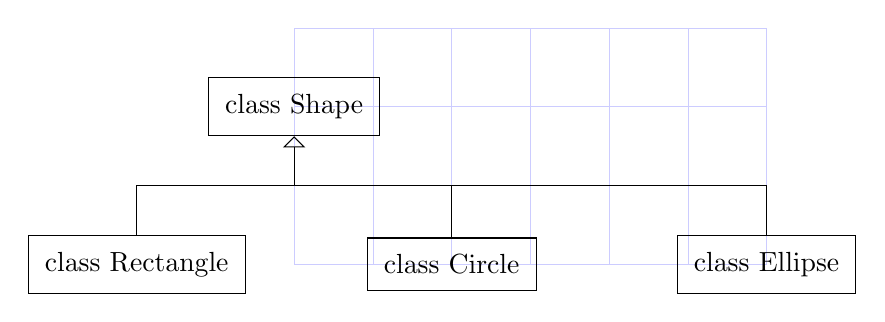
\begin{tikzpicture}[shapeName/.style={inner sep=6pt}]
\path[help lines, blue!20, draw] (0,0) grid (6, 3);
	\node[shapeName] (shape) at (0,2) [draw] {class Shape};
	\node[shapeName] (rect) at (-2,0) [draw] {class Rectangle};
	\node[shapeName] (circle) at (2,0) [draw] {class Circle};
	\node[shapeName] (ellipse) at (6,0) [draw] {class Ellipse};
	\draw (node cs:name=circle,anchor=north) |- (0,1);
	\draw (node cs:name=ellipse,anchor=north) |- (0,1);
	\draw[-open triangle 90] 
		(node cs:name=rect,anchor=north)
		|- (0,1) 
		-| (node cs:name=shape,anchor=south);
\end{tikzpicture}

\end{document}